\chapter{Inhalt}

Im laufe dieser Arbeit wurden verschiedene Algorithmen zur lokalen Merkmalsextraktion und Deskriptorberechnung getestet und ausgewertet.
Das Ziel ist hierbei Merkmale zu finden die so gut wie möglich folgenden Ansprüchen genügen und somit als stabil bezeichnet werden:
\begin{itemize}
\item \emph{Skaleninvarianz}: Unabhängigkeit von der Größe auf dem Bild (Distanz zur Kamera)
\item \emph{Rotationsinvarianz}: Merkmale können trotz einer Rotation erkannt werden
\item \emph{Beleuchtungsinvarianz}: Ermöglicht Erkennung der Merkmale bei verschiedenen Lichtverhältnissen
\item \emph{Blickwinkelunabhängigkeit}: Unabhängigkeit von der Position aus der das Objekt aufgenommen wird
\end{itemize} 

\section{SIFT}

Die "Scale Invariant Feature Transform" ist bis heute eine der erfolgreichsten Methoden zur lokalen Merkmalsextraktion. Sie wurde 1999 von David Lowe vorgestellt und ist von der Objekterkennung im menschlichen Gehirn inspiriert.

\subsection{Merkmalsextraktion}

Aus dem zu untersuchenden Bild wird als erstes der sogenannte \emph{scale-space} berechnet.

\begin{figure}[h]
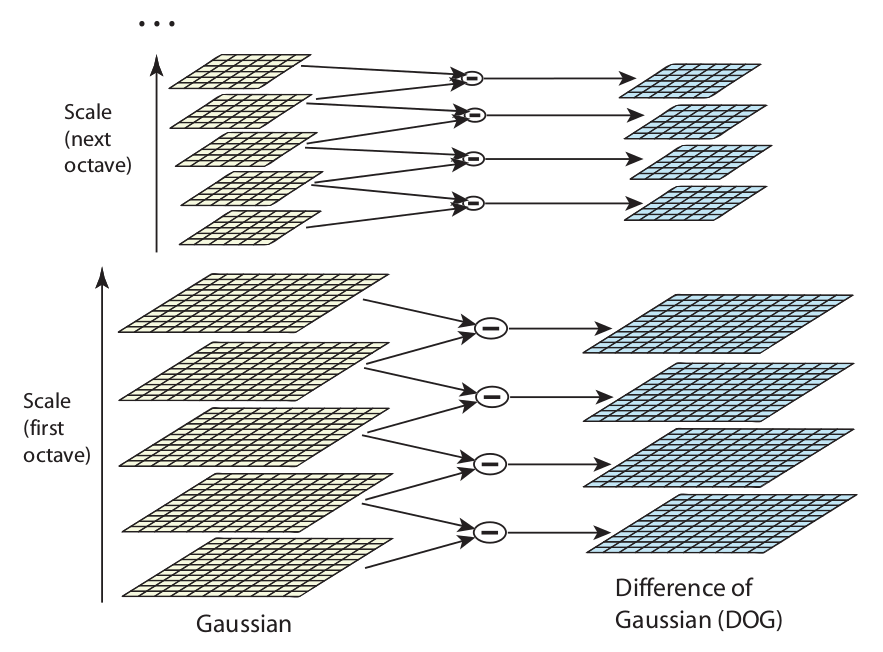
\includegraphics[width=0.6\textwidth]{scale_space.png}
\centering
\end{figure}
Hierzu wird das Bild mit einem Gauss-Kernel wiederholt geglättet um die \emph{scales} der ersten \emph{octave} zu erstellen.
Um die Gaussgeglätteten Bilder $ L (x, y, \sigma ) $ zu erhalten wird der Gauss-Kernel 
\begin{equation}
G(x, y, \sigma) = \frac{1}{2\pi\sigma^{2}}e^{-(x^{2}+y^{2})/2\sigma^{2}}
\end{equation}
 mit dem Ursprungsbild $ I(x, y) $ gefaltet:
\begin{equation}
L(x, y, \sigma) = G(x, y, \sigma)\ast I(x, y)
\end{equation}
Hiermit werden schrittweise immer mehr kleine Merkmale entfernt, was dazu führt dass größere Merkmale and Bedeutung gewinnen.
Die Breiten der Gaussfunktionen mit der zwei benachbarte \emph{scales} berechnet werden, haben das konstante Verhältnis $ k $, hierdurch sind die \emph{scales} im \emph{scale-space} equidistant in Bezug auf $ \sigma $.

Lowe fand experimentell heraus, dass die optimale Anzahl an \emph{scales} per \emph{octave}, in Bezug auf die Wiederholgenauigkeit der Detektion der Merkmale nach verschiedenen Bildtransformationen, 3 beträgt.
\begin{figure}[h]
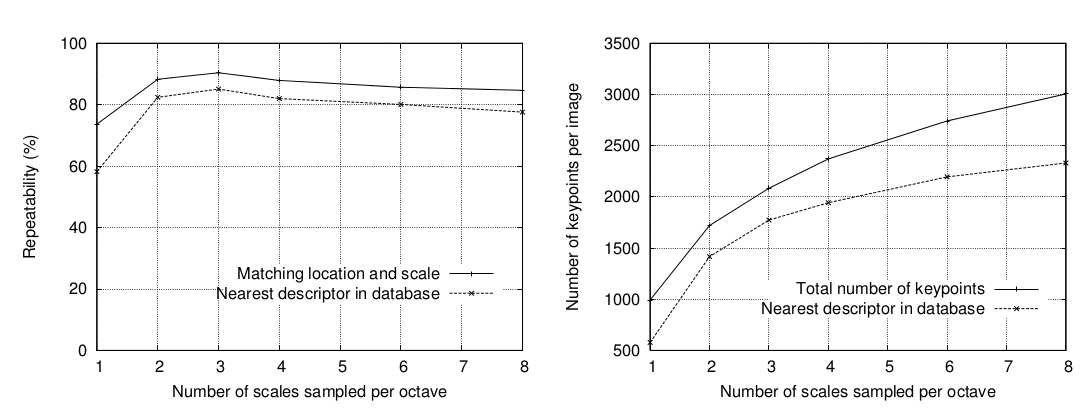
\includegraphics[width=0.6\textwidth]{scale_number.png}
\centering
\end{figure}
Nachdem die \Glspl{scale} der ersten \Gls{octave} berechnet wurden, wird das Bild mit dem doppelten Initialwert von $ \sigma $ runterskaliert in dem jedes zweite Pixel jeder Reihe und jeder Spalte beibehalten wird. Das erhaltene Bild ist der erste \Gls{scale} der nächsten \Gls{octave} aus dem die darauf folgenden wie zuvor erstellt werden.
In der folgenden Abbildung ist das Ergebnis dieses Vorgangs veranschaulicht.

\begin{figure}[h]
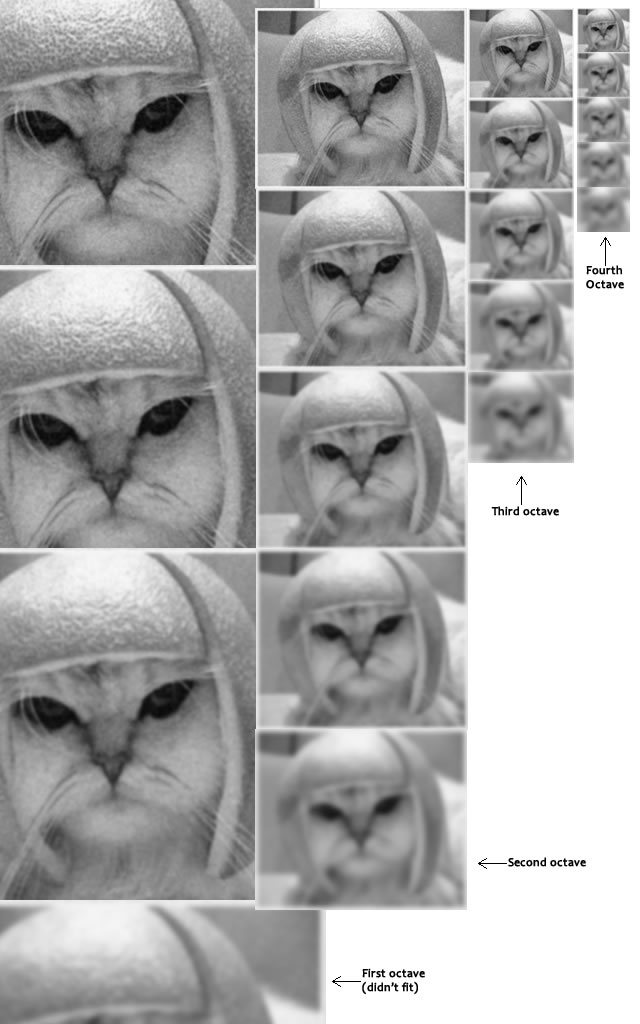
\includegraphics[width=0.4\textwidth]{sift-octaves.jpg}
\centering
\end{figure}

Um die Merkmale zu finden, werden die lokalen Extrema der \emph{Difference of Gaussian} Funktion zwischen den benachbarten \Glspl{scale} berechnet. Mikolajczyk fand in experimentellen Vergleichen mit anderen Bildfunktionen, wie der Gradient, der Hesse- und der Harrisfunktion heraus, dass diese Methode die stabilsten Merkmale extrahiert.

Als erstes werden hierzu die \emph{Difference of Gaussian} zwischen den verschiedenen Ebenen des \Gls{scale-space}s ermittelt:	
\begin{equation}
D(x, y, \sigma) = (G(x, y, k\sigma) - G(x, y, \sigma)) \ast I(x, y)
= L(x, y, k\sigma) - L(x, y, \sigma)
\end{equation} 

Um die Lokalen Maxima zu finden, wird jedes Pixel mit den 8 benachbarten im selben \Gls{scale} und den 9 benachbarten in den darüber und darunter liegenden \Glspl{scale} verglichen. Stellt das Pixel ein Maximum oder ein Minimum in der betrachteten Menge von Pixeln dar, stellt es einen potentiellen \emph{Keypoint} da.

\begin{figure}[h]
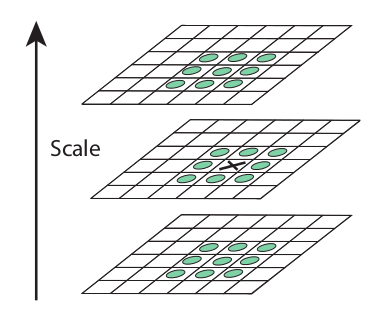
\includegraphics[width=0.4\textwidth]{sift_maxima.png}
\centering
\end{figure}

Um nur die stabilsten \emph{Keypoints} beizubehalten wurde von Brown vorgeschlagen mit Hilfe der quadratischen Taylorexpansion die Position der Keypoints auf Subpixel-Genauigkeit zu bestimmen.
Außerdem werden auch Keypoints mit einem niedrigen Kontrast gefiltert.

Da die Suche nach Keypoints mit der \emph{Difference of Gaussian} Funktion an den Kanten viele unsignifikante Punkte liefert werden anschließend die Gradienten der Punkte in x und y-Richung und deren Verhältnis $ r $ berechnet. Ist dieses größer als ein Schwellwert (Lowe verwendet r=10) wird der Keypoint gelöscht.

Um die Keypoints Rotationsinvariant zu machen wird ihnen eine Richtung zugewiesen. Lowe hat herausgefunden dass sich hierzu die Orientierung der Bildpunkte um den Keypoint gut eignet. 
Er berechnet die Größe und die Orientierung der Gradienten der umliegenden Pixel im \Gls{scale} des jeweiligen Keypoints:
\begin{equation}
m(x, y) = \sqrt{(L(x + 1, y) - L(x - 1, y))^{2} + (L(x, y + 1) - L(x, y - 1))^{2}}
\end{equation}
\begin{equation}
\Theta (x, y) = tan^{-1}((L(x, y + 1) - L(x, y - 1))/(L(x + 1, y) - L(x - 1, y)))
\end{equation}
Die Orientierungen werden anschließend mit den Größen gewichtet und in 36 \"bins\" eines Histogramms unterteilt. Dem Keypoint wird die häufigste Orientierung des Histogramms zugewiesen und zusätzlich wird ein Keypoint mit jeder Orientierung die mindestens 80\% der maximalen Häufigkeit besitzt erstellt.

\subsection{Deskriptorberechnung}

Um die Keypoints zu charakterisieren wird ein sogenannter \emph{Deskriptor} berechnet.
Hierzu werden die Gradientengrößen und Orientierungen eines 16x16 Pixel Feldes um den Keypoint herum bestimmt und mit der Gaussfunktion gewichtet um den Einfluss weiter entfernter Punkte zu verringern.
Die Rotationsinvarianz des \emph{Deskriptors} wird erreicht in dem die Orientierungen der Gradienten relativ zur Orientierung des Keypoints gedreht werden.

\begin{figure}[h]
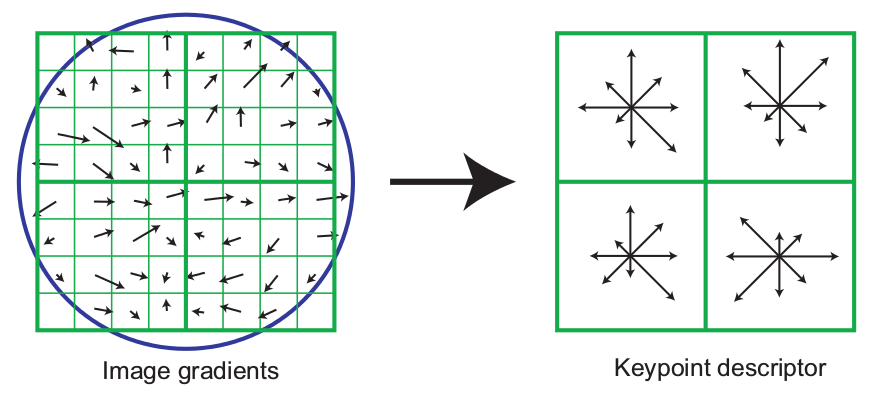
\includegraphics[width=0.8\textwidth]{sift_orientation.png}
\centering
\end{figure}

Die Pixel werden in 4x4 Pixel große Felder unterteilt und innerhalb dieser werden wie bei der Orientierungsbestimmung der Keypoints die gewichteten Werte der Gradienten in Histogramme akkumuliert. Diese besitzen 8 \"bins\" die den Orientierungen entsprechen. Zusätzlich werden die Gradienten trilinear interpoliert indem sie nach einer Gewichtung in Abhängigkeit der Distanz auch auf die benachbarten Histogramme aufsummiert werden. Dadurch entsteht bei der Wiedererkennung der Merkmale ein bestimmtes Maß an Toleranz, dass die Erkennung von Objekten aus einem anderen Sichtwinkel oder nach einer nicht-starren Deformation ermöglicht.

Die \emph{Deskriptoren} werden als Vektoren gespeichert, die alle $4x4x8=128$ Werte der \"bins\" der Histogramme enthalten. 
Die Merkmale sind gegen Helligkeitsveränderungen die gleichermaßen alle Pixel aus denen sie berechnet wurden betreffen stabil, da die Gradienten durch Differenzen gebildet werden.
Um Stabilität gegen Kontrastveränderungen zu erreichen wird der Merkmalsvektor normiert.
Um den Einfluss von nicht linearen Helligkeitsveränderungen zu verringern, werden alle Werte des Vektors die Größer als 0.2 sind auf diesen Wert gesetzt. Anschließend wird der Vektor nochmals normiert. \cite{lowe99}


\section{SURF}

Nachdem es mit SIFT und anderen Algorithmen möglich war sehr charakterisierende und somit mit sehr hoher Wiederholgenauigkeit erkennbare Merkmale aus Bildern zu extrahieren, kam das Bedürfnis nach einer Lösung die weniger rechenintensiv ist auf um Merkmalserkennung auch in \Glspl{Online-System}n anzuwenden.
Mit diesem Ziel entwickelten H. Bay, T. Tuytelaars und L. Van Gool die \"Speeded Up Robust Features\", kurz SURF, und veröffentlichten diese im Jahr 2006.

\subsection{Merkmalsextraktion}

Der Detektor von SURF-Merkmalen basiert auf der Hesse-Matrix, diese enthält die zweiten Ableitungen der 2D-Gaussfunktion:
\begin{equation}
H(x, \sigma) =
\begin{bmatrix}
L_xx (x, \sigma) & L_xy (x, \sigma) \\
L_xy (x, \sigma) & L_yy (x, \sigma)
\end{bmatrix}
\end{equation}
Es wird die Determinante dieser benutzt um die Position und den Scale der Keypoints zu detektieren.
Diese wird anschließend noch durch die Varianz der Gaussfunktion geteilt um das Ergebnis zu normalisieren:
\begin{equation}
DoH(x, y, \sigma)=\dfrac{G_{xx}(x, y, \sigma)\cdot G_{yy}(x, y, \sigma)-G_{xy}(x, y, \sigma)^{2}}{\sigma^{2}}
\end{equation}

Statt wie bei den SIFT-Merkmalen den Laplacian of Gaussian durch die Difference of Gaussian zu approximieren, verwenden die Autoren des SURF Verfahrens den Rechteck Filter.

\begin{figure}[h]
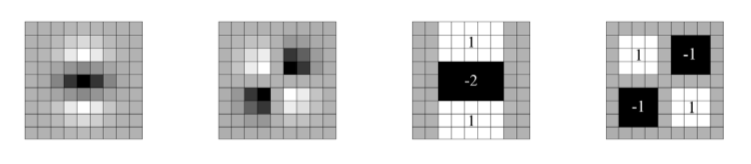
\includegraphics[width=0.9\textwidth]{surf_boxfilter.png}
\centering
\end{figure}

Dieser ist zwar nicht so genau, aber dafür durch die Benutzung von Integralbildern viel schneller zu berechnen.
Jede Position $X=(x, y)$ des Integralbildes beinhaltet die Summe aller Pixel aus dem Originalbild die innerhalb des durch die Position $X$ und den Ursprung aufgespannten Rechtecks liegen:
\begin{equation}
I_\Sigma(X)=\sum_{i=0}^{i\leq x}\sum_{j=0}^{j\leq y}I(x,y)
\end{equation}

Ein weiterer Geschwindigkeitsvorteil wird dadurch erzielt dass der Scale-Space nicht im Voraus berechnet werden muss. Durch die Integralbilder sind die Kosten der Berechnung der Rechteckfilter nicht von der Größe der Maske abhängig und somit können die verschiedenen \Glspl{scale} durch die Anpassung der Maskengröße simuliert werden und das Originalbild muss für die verschiedenen \Glspl{octave} nicht mehr verkleinert werden.

\subsection{Deskriptorberechnung}

Der SURF Desktriptor ist von der Grundidee dem SIFT-Deskriptor sehr ähnlich.
Auch hier wird als erstes die Orientierung extrahiert und dann das Merkmal durch sein Umfeld charakterisiert.
Hierzu verwendet SURF allerdings Haar Wavelets da diese sehr schnell berechenbar sind.

Um die Orientierung zu bestimmen werden ein horizontales und ein vertikales Haar Wavelet in einem Umkreis von $6s$ um das Merkmal in dem entsprechenden Scale $s$ des Merkmals berechnet.
Auch hier wird auf Integralbilder zurückgegriffen da die Wavelets eine Seitenlänge von $4s$ haben und somit für größere Scales sehr groß werden.
Der Umkreis des Merkmals wird in Abschnitte mit einer Breite von $\dfrac{\pi}{3}$ unterteilt und in jedem werden die Ergebisse des Horizontalen Wavelets und anschließend die des Vertikalen aufsummiert.
Somit erhält jeder Abschnitt ein Orientierungsvektor und der mit dem größten Betrag wird als Orientierung des Merkmals verwendet.

Um den Deskriptor zu extrahieren wird ein Quadrat mit $20s$ Seitenlänge, das nach der vorher bestimmten Orientierung ausgerichtet ist, um das Merkmal gespannt.
Dieses wird in 4 gleichgroße Unterbereiche unterteilt und in jedem dieser werden die Horizontalen und Vertikalen (in Bezug auf die Orientierung des Merkmals) Haar-Wavelets $d_x$ und $d_y$ für 5x5 gleichmäßig verteilte Punkte ermittelt. 
Die Ergebnisse der Haar-Wavelets werden dann aufsummiert und zusätzlich werden noch die Beträge der einzelnen Komponenten aufsummiert.
Hiermit erhält man einen vierdimensionalen Vektor für jeden der 16 Unterbereiche:
\begin{equation}
v=(\sum d_x, \sum d_y, \sum |d_x|, \sum |d_y|)
\end{equation}
Wie diese Methode eine Charakterisierende Beschreibung für das Umfeld eines Merkmals ist beschreiben die Autoren im folgenden Bild.

\begin{figure}[h]
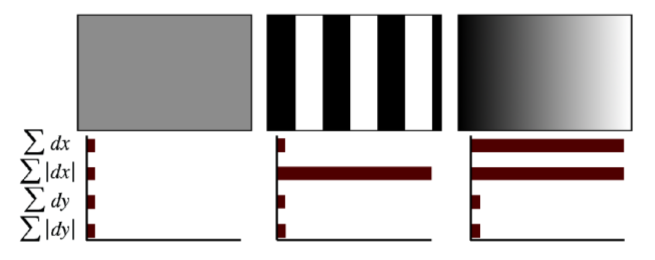
\includegraphics[width=0.8\textwidth]{surf_descriptor_expl.png}
\centering
\end{figure}

Wie auch der Merkmalsvektor bei SIFT, ist dieser bei SURF invariant gegenüber globalen Beleuchtungsveränderungen. Auch hier wird eine Kontrastinvarianz durch die Normierung erzielt. 
\cite{bay08}

\section{ORB}

Ein weiterer Algorithmus um effizient Merkmale aus Bildern zu extrahieren wurde von Edward Rosten und Tom Drummond unter dem Namen ORB vorgestellt.
ORB steht für \emph{Oriented FAST and Rotated BRIEF} da die Merkmalslokalisierung auf FAST basiert und die Deskriptorbeschreibung eine verbesserte Version von BRIEF ist.

\subsection{Merkmalsextraktion}
Um die Funktionsweise von Oriented FAST besser zu beschreiben wird im folgenden der darunterliegende Algorithmus FAST erläutert.
\subsubsection{FAST}

Der \emph{Features from Accelerated Segment Test} (FAST) ist vom Segment Test abgeleitet.

\begin{figure}[h]
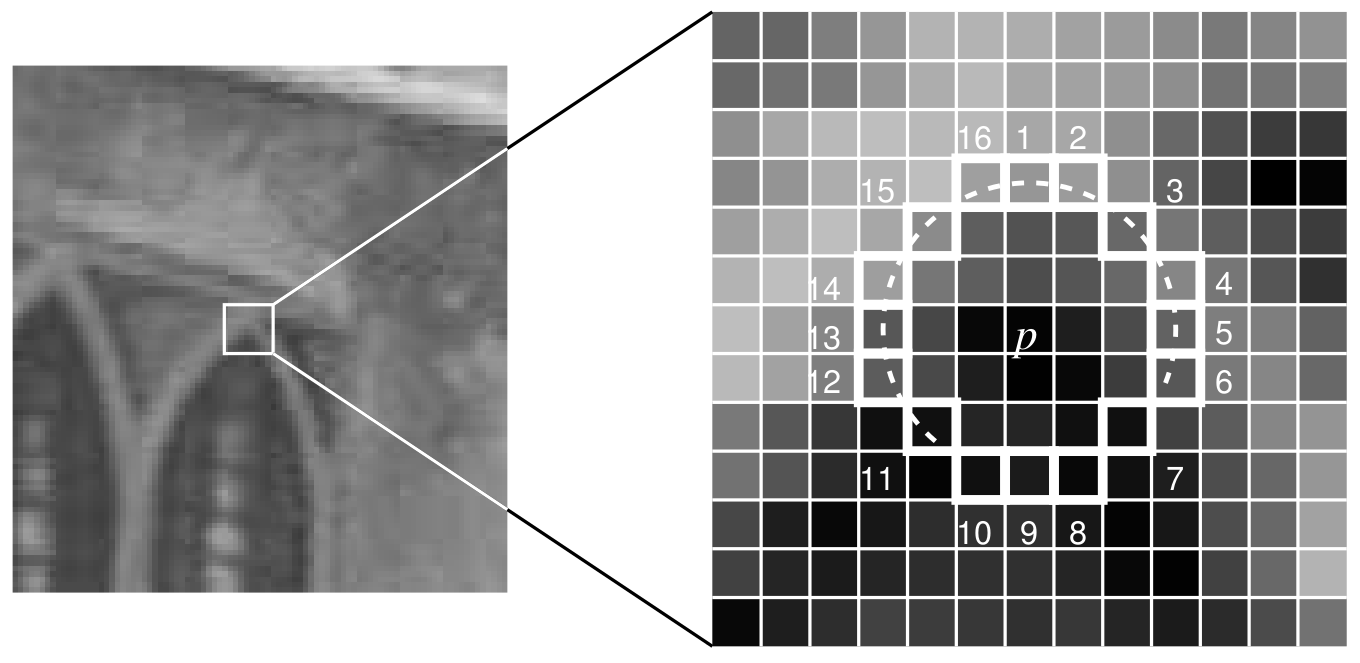
\includegraphics[width=0.8\textwidth]{segment_test.png}
\centering
\end{figure}

Dieser untersucht das Umfeld der einzelnen Punkte im Bild in dem er den umliegenden Kreis mit 16 Pixeln Länge mit dem Zentrum vergleicht.
Um möglichst schnell viele Bildpunkte raus zu filtern werden vorerst nur die Pixel 1, 5, 9 und 13 berücksichtigt und nur Punkte bei den 3 von diesen Pixeln heller oder dunkler als der berücksichtigte Bildpunkt sind als Kandidaten genommen.
Die Bildpunkte die den ersten Test bestehen werden anschließend genauer analysiert in dem jedes Pixel des umliegenden Kreises mit dem Zentrum verglichen wird.
Wenn der Kreis eine zusammenhängende Kette von 12 Pixeln die heller oder dunkler als der zugehörige Bildpunkt sind beinhaltet, wird dieser als Merkmal hinterlegt.
Um diesen Vorgang zu optimieren wird bei FAST von maschinellem lernen gebrauch gemacht: es wird ein \emph{Decision Tree} wie von Quinlan in \emph{Induction of Decision Trees} beschrieben aufgebaut.
Um das System einzulernen wird ein Set aus Bildern genutzt, die bestenfalls dem Typ von Umgebung entsprechen in dem das Bildverarbeitungssystem eingesetzt werden soll.
Jedes Pixel dieser Bilder wird mit jedem Punkt $ x \in {1..16} $ des umliegenden Kreises verglichen um dann jedem Kreispunkt einen Zustand zuzuweisen:
\begin{equation}
S_{p\rightarrow x}=
\begin{cases}
d, & \quad I_{p\rightarrow x}\leq I_p - t\\
s, & \quad I_p - t < I_{p\rightarrow x} < I_p + t\\
b, & \quad I_p + t \leq I_{p\rightarrow x}
\end{cases}
\end{equation}
wobei $I_p$ die Intensität des Bildpunktes und $I_{p\rightarrow x}$ die Intensität des Pixels an der Stelle x auf dem Kreis um $I_p$ ist.
Anhand dieses Zustands werden alle Pixel $p$ der Menge $P$ aller Bildpunkte der Trainings-Bilder in die 3 Untermengen $P_d$, $P_s$ und $P_b$ unterteilt.
Um das $x$ zu bestimmen welches am besten aussagt ob ein Pixel eine Ecke ist, wird die Entropie der Ecken-Eigenschaft $K$ (bei Pixeln  $p$ die als Ecke erkannt wurden hat $K_p$ den Wert 1) in den Mengen $P$,$P_d$, $P_s$ und $P_b$ berechnet.
Hieraus wird der Informationsgewinn berechnet als:
\begin{equation}
H(P) - H(P_d) - H(P_s) - H(P_b)
\end{equation}
Das $x$ mit dem höchsten Informationsgewinn wird zur Unterteilung von $P$ in seine Teilmengen verwendet.
Dieser Vorgang wird so lange wiederholt bis die Entropie einer der Untermengen zu $0$ wird und somit entweder nur oder keine Ecken enthält.
\subsubsection{Oriented FAST}
Da FAST keine Orientierungskomponente hat ist der Algorithmus nicht rotationsinvariant.
Um dieses Problem zu beheben wird von dem \emph{Intensitäts-Schwerpunkt} Gebrauch gemacht da dieser bei einer Ecke nie mit dem Mittelpunkt übereinstimmt.
Dieser Schwerpunkt wird wie folgt berechnet:
\begin{equation}
C = (\dfrac{m_{10}}{m_{00}}, \dfrac{m_{01}}{m_{00}})
\end{equation}
mit den Momenten:
\begin{equation}
m_{pq} = \sum_{x,y}x^p y^q I(x,y)
\end{equation}

Dem Merkmal wird dann die Orientierung des Vektors der vom Mittelpunkt des Winkels $O=(0,0)$ zum \emph{Intesitäts-Schwerpunkt} zeigt zugewiesen:
\begin{equation}
\Theta = atan2(m_{01},m_{10})
\end{equation}

Um die Rotationsinvarianz zu optimieren, werden die Momente nur aus Pixeln berechnet deren x und y Werte innerhalb eines durch den Radius r um den Mittelpunkt aufgespannten Kreises liegen.

Bild Intensitätsschwerpunkt?


\subsection{Deskriptorberechnung}

\subsubsection{BRIEF}
BRIEF ist eine Methode zur Merkmalsextraktion die gegenüber SURF noch einen Schritt weiter in der Rechenzeitoptimierung geht. Hierzu verwenden die Authoren die Erkenntnisse der Arbeiten \emph{Fast Keypoint Recognition Using Random Ferns} und \emph{Keypoint Recognition Using Randomized Trees}.
Diese haben gezeigt das Teile eines Bildes effektiv durch wenige Vergleiche der Intensität in Pixelpaaren beschrieben werden können. 
Um einen BRIEF Deskriptor zu berechnen wird der folgende Test $\tau(p;x,y)$ auf die zu untersuchenden Pixelpaare angewandt und die Binären Ergebnisse in einem Vektor gespeichert:
\begin{equation}
\tau(p;x,y)=
\begin{cases}
1, & \quad \text{if } p(x) < p(y)\\
0, & \quad \text{otherwise}
\end{cases}
\end{equation}
Um die Störungsanfälligkeit zu reduzieren wird das Bild davor mit einem Gaussfilter geglättet.
Um den Filter effektiv zu nutzen haben die Autoren die drei Einflussgrößen experimentell bestimmt:
\begin{itemize}
\item \emph{Kernel des Gaussfilters}: Nachdem verschiedene Gausskurvenbreiten $\sigma$ zwischen 0 und 3 getestet wurden, hat sich $\sigma=2$ als die beste Wahl herausgestellt. Als Größe des Kernels wurde 9x9 Pixel genommen.

\item \emph{Räumliche Anordnung der Tests}: Wie die Versuche mit verschiedenen Strategien zur bestimmung der Anordnung der Tests gezeigt haben, spielt diese eine wichtige Rolle für die Güte (Wiedererkennungsrate) der Deskriptoren.
Folgende Anordnungen wurden verglichen:
\begin{figure}[h]
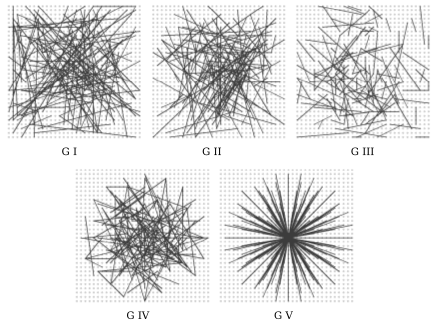
\includegraphics[width=0.6\textwidth]{brief_distribution.png}
\centering
\end{figure}

Die ergebnisse des Vergleichs sind im folgenden Graphen zu sehen:
\begin{figure}[h]
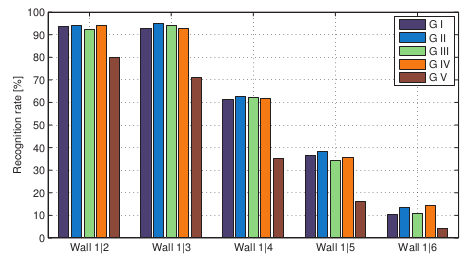
\includegraphics[width=0.6\textwidth]{brief_placement_results.png}
\centering
\end{figure}
Die symmetrische Anordnung ist mit Abstand die schlechteste und die Zweite ist in den meisten Fällen ein bisschen im Vorsprung gegenüber dem Rest, daher wird diese verwendet.
Es handelt sich hierbei um eine isotropische Gaussverteilung mit $\sigma^2=\frac{1}{25}S^2$ wobei $S$ die Seitenlänge des zu betrachtenden viereckigen Bildausschnitts ist.

\end{itemize}

\subsubsection{Rotated BRIEF}
BRIEF besitzt eine sehr schlechte Rotationsinvarianz, daher wurde für ORB die Variante Rotated BRIEF entworfen.
Für das Set aus Tests zur Erstellung des Deskriptorvektors an den stellen $(x_i, y_i)$ wird diese Matrix definiert:
\begin{equation}
S=
\begin{pmatrix}
x_1 & \cdots & x_n \\
y_1 & \cdots & y_n
\end{pmatrix}
\end{equation}

Anschließend wird die der Orientierung $\Theta $ des Merkmals entsprechende Rotationsmatrix $R_\Theta$ verwendet um $S_\Theta $ wie folgt zu berechnen:
\begin{equation}
S_\Theta = R_\Theta \cdot S
\end{equation}
$\Theta$ wird auf Abschnitte mit einer Breite von $\dfrac{2\pi}{30}$ diskretisiert und es wird eine Lookup-Tabelle mit den Positionen der zu testenden Punkte für jeden Diskretisierungsschritt im fertigen Programm hinterlegt.
Somit lassen sich die rotationsunabhängigen Deskriptoren praktisch genauso schnell wie die rotationsabhängigen berechnen. \cite{rub11}

\section{Bruteforce Matcher}
Der \emph{Bruteforce Matcher} ist ein von Opencv bereitgestelltes Werkzeug um Übereinstimmungen zwischen extrahierten Merkmalen zu finden. 
Hierzu wird die sogenannte Distanz zwischen den jeweiligen Deskriptoren der Merkmale berechnet.
Dieser Wert ist ein Maß für die Änlichkeit zweier verglichener Deskriptoren und somit die Wahrscheinlichkeit dass die zugehörigen Merkmale Übereinstimmen.
Diese Distanz wird durch die Differenz verschiedener Vektornormen bestimmt.
Die Wahl des richtigen Algorithmus hängt unter anderem von dem Typ des Deskriptors ab (Fließkomma- oder Binärwerte) und kann durch den Parameter \emph{normType} festgelegt werden. Es stehen folgende Vektornormen zu Verfügung:
\begin{itemize}
\item \emph{NORM\_L1}
\item \emph{NORM\_L2}
\item \emph{NORM\_HAMMING1}
\item \emph{NORM\_HAMMING2}
\end{itemize}

Für das Matching der SIFT und SURF Deskriptoren wird in dieser Arbeit die \emph{NORM\_L2} verwendet.
Diese auch unter dem Namen \emph{Euclidische Norm} bekannte Größe wird nach folgender Formel berechnet:
\begin{equation}
\ell^2 = ||x|| = \sqrt{\sum_{k=1}^{n}|x_k|^2}
\end{equation}

wobei $|x_k|$ der Betrag der komplexen Zahl $x_k$ ist und somit für Deskriptoren mit rein reellen Zahlen (wie SIFT und SURF) $|x_k|^2 = x_k^2$ ist.

Um das Matching der ORB Deskriptoren durchzuführen wird von \emph{NORM\_HAMMING1} gebrauch gemacht.
Es handelt sich nicht um eine Vektor-Norm im engen Sinn wird aber manchmal als eine solche bezeichnet.
Diese Größe ist auch als \emph{Hamming Distanz} bekannt und ist die Anzahl unterschiedlicher Bits in zwei gleich langen Bit-Ketten.
Hierzu werden alle Positionen in den zwei Ketten stellenweise verglichen und falls die Werte nicht übereinstimmen die \emph{Hamming Distanz} um 1 erhöht. 

\begin{figure}[h]
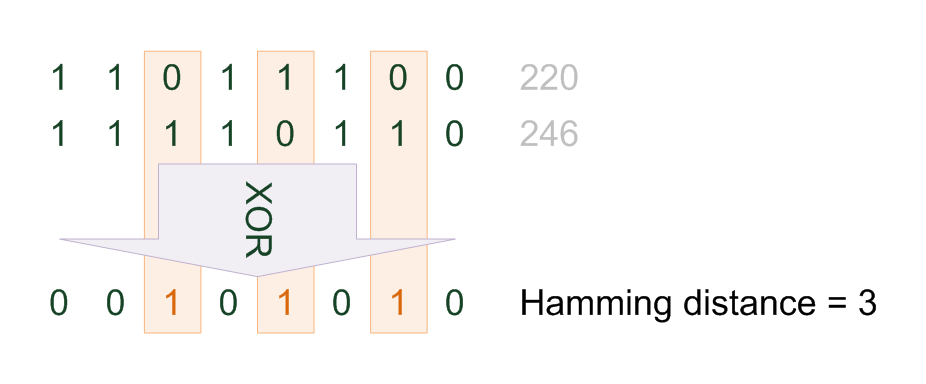
\includegraphics[width=0.6\textwidth]{hamming.png}
\centering
\end{figure}

Diese Operation kann mit minimalen Kosten berechnet werden da es genügt die beiden Bit-Ketten mit einem \emph{XOR} Operator zu vergleichen und die positiven Bits zu zählen. \cite{cvman}

\section{Homographie}
Homographie ist der mathematische Zusammenhang von zwei 2-Dimensionalen Abbildungen eines 3-Dimensionalen Objekts.
Die Berechnung um diese zu finden wird in $P^2$, der homogenen Darstellung, durchgeführt.
Ein Punkt $P'\in \mathbb{R}$ in kartesischer Darstellung kann aus dem Punkt $P \in \mathbb{P}$ in homogener Darstellung durch die folgenden Beziehungen abgeleitet werden:
\begin{equation}
x' = \dfrac{x}{z} \quad \text{und} \quad y' = \dfrac{y}{z}
\end{equation}
Umgekehrt wird $P$ aus $P'$ wie folgt bestimmt:
\begin{equation}
P' = 
\begin{pmatrix}
    x'\\
    y'
\end{pmatrix}
\quad \rightarrow \quad
P = 
\begin{pmatrix}
    x\\
    y\\
    1
\end{pmatrix}
\end{equation}

Hartley und Zisserman bezeichnen die Homographie wie folgt\:

Ein Zusammenhang von $\mathbb{P}^2 \quad \rightarrow \quad \mathbb{P}^2$ ist eine Homographie wenn eine nicht singuläre 3x3 Matrix $H$ existiert sodass aus jedem Punkt $x$ der zusammenhängende als $Hx$ berechnet werden kann. \cite{harzis}

\section{RANSAC}
\emph{Random Sample Consensus} ist ein Algorithmus um die Übereinstimmung von einem mathematischen Modell mit Testdaten zu überprüfen und somit das sogenannte Matching durchzuführen.
Das zuvor verbreitete Matchingverfahren \emph{Least Median of Squares Regression} berücksichtigte für die Auswertung die Gesamtheit der Testdaten und konnte somit nur auf Testdaten mit einem Ausreißeranteil der kleiner als 50\% ist angewandt werden.
Hierfür wurde RANSAC entwickelt.
Es wird zunächst eine Teilmenge S1, mit der minimalen Anzahl an Punkten um die nötigen Parameter der Modellfunktion zu berechnen, zufällig aus der Menge der Testdaten P gewählt. 
Anschließend wird das \emph{Consensus Set} S1* aus Punkten die innerhalb einer Tolleranzgrenze dem gefundenen Modell entsprechen bestimmt.
Wenn diese Menge eine gewisse Mindestanzahl an Punkten enthält wird es als Kandidat für die Lösung genommen.
Diese schritte werden mehrmals wiederholt um die Modellhypothese mit dem Größten Consensus Set zu finden.
Hierbei ergeben sich drei Parameter für RANSAC:
\begin{itemize}
\item \emph{Zugelassene Fehlertoleranz um ein Punkt in ein Consesus Set aufzunehmen}
\item \emph{Anzahl der Iterationen}
\item \emph{Mindestanzahl der Punkte in einem Consesus Set}
\end{itemize}
\cite{fis80}